\section{Theorie}
\label{sec:Theorie}
Unter einer Spannungsquelle ist ein elektrisches Bauteil zu verstehen,
welches für eine endliche Zeit eine konstante Spannung bereitstellen kann. Stellt die
Spannungsquelle keinen Strom zur Verfügung, so liegt an ihr die sogenannte Leerlaufspannung
$U_0$ an. Wird ein Lastwiderstand mit dem Widerstand $R_\text{a}$ mit
einer realen Spannungsquelle in Reihe geschaltet, dann fällt am Lastwiderstand
eine Klemmenspannung $U_\text{K}$ ab, die geringer als die Leerlaufspannung $U_0$
ist. Dies lässt sich dadurch erklären, dass die reale Spannungsquelle einer
idealen Spannungsquelle entspricht, die mit dem Innenwiderstand
$R_\text{i}$ in Reihe geschaltet ist. Die ideale Spannungsquelle ist in der Lage,
eine konstante Spannung $U_0$ bei einem Innenwiderstand von null zu liefern.
Die dann vorliegende Schaltung ist in Abbildung \ref{fig:ersatzschaltbild} zu sehen.

\begin{figure}
  \centering
  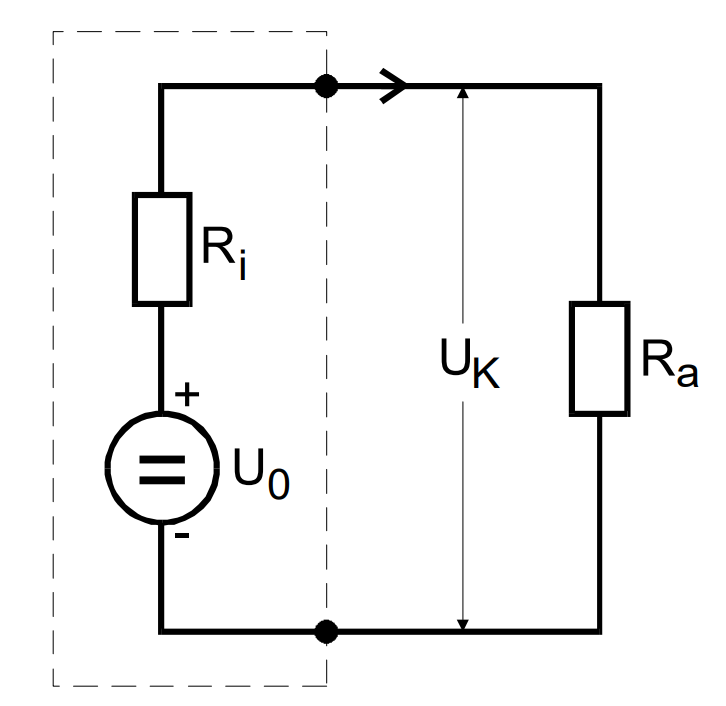
\includegraphics[width=150pt]{data/ersatzschaltbild.png}
  \caption{Schaltbild einer realen Spannungsquelle und eines Lastwiderstands in Reihe \cite{Versuchsanleitung}}
  \label{fig:ersatzschaltbild}
\end{figure}

Um Informationen über die Beziehungen zwischen den Größen in dieser Schaltung zu erhalten,
wird die Kirchhoffsche Maschenregel angewandt: Die Summe aller Spannungen in einer
Masche addiert sich zu null, das bedeutet also
\begin{equation}
  \sum\limits_{k=1}^N U_k = 0\,,
  \label{eqn:kirchhoffmasche}
\end{equation}
falls an der Masche insgesamt $N$ Teilspannungen abfallen.
Nach Anwendung dieser Formel auf diese konkrete Schaltung ergibt sich die Zuordnung
\begin{equation}
  U_\text{K}(I) = I R_\text{a} = U_0 - I R_\text{i}
  \label{eqn:klemmevoni}
\end{equation}
für die Klemmenspannung in Abhängigkeit der Stromstärke $I$. Wird eine Spannung durch
einen Voltmeter gemessen, dann verfügt dieses für gewöhnlich über einen hohen Widerstand,
sodass der Stromfluss näherungsweise null beträgt und der zweite Summand vernachlässigt
werden kann.
In diesem Grenzfall gilt $U_0 \approx U_\text{K}$, die abzulesende
Klemmenspannung ist ungefähr gleich der Leerlaufspannung der Spannungsquelle.

Für die Leistung $P$, die an einem Lastwiderstand $R_\text{a}$ umgesetzt wird,
gilt
\begin{equation}
  P = I^2 R_\text{a}\,.
  \label{eqn:leistung}
\end{equation}
Diese Leistung kann nicht beliebig groß werden. Stattdessen durchläuft sie ein
Maximum. Der Versuch, die maximale Leistung am Verbraucher umzusetzen, wird als
Leistungsanpassung bezeichnet. Dies kann hier erreicht werden, indem $R_\text{a}$
geeignet gewählt wird.

Im Allgemeinen liegt kein linearer Zusammenhang zwischen den betrachteten Größen vor.
Dies ist insbesondere der Fall, wenn statt Gleichstrom ein Wechselstrom anliegt.
Dann ist der Quotient $\frac{U}{I}$ nicht konstant und der Innenwiderstand ist
die differenzielle Größe
\begin{equation}
  R_\text{i} = \frac{\symup{d} U_\text{K}}{\symup{d} I}\,.
  \label{eqn:differentiell}
\end{equation}
